\chapter{Chapter title}

\begin{bf}
  \author{Author Name}\\
  
Abstract\\
\end{bf}

This chapter discusses some important things


\section{A Section}

Lorem ipsum dolor sit amet, consectetur adipiscing elit. Duis eu egestas erat. Maecenas tincidunt lacinia tincidunt. Mauris id lectus nec neque feugiat condimentum vitae at diam. In vel orci nunc, non commodo mauris. Vivamus ipsum enim, vulputate quis pharetra non, molestie quis felis. Vivamus porttitor placerat turpis at accumsan. Nunc tortor velit, faucibus a rhoncus nec, blandit non elit. Nam consectetur lectus eu nisi blandit dapibus rhoncus dui tempus. Mauris fermentum dolor vel ipsum vulputate sit amet ultricies tortor lacinia. Donec ut nibh erat. Morbi nec mi ante. Integer nec vestibulum diam. Donec tincidunt pellentesque quam, ut interdum mauris venenatis condimentum. Nam condimentum, augue in aliquet gravida, neque dui elementum eros, id semper eros purus sed felis. Curabitur in justo sit amet sapien ultrices hendrerit at quis nibh. Quisque iaculis pulvinar tincidunt. 
\begin{eqnarray}
C(12) &= &\left[\overrightarrow{\pi}\cdot\overrightarrow{\phi}(x+r)\right] \nonumber \\ 
&\approx& 1-\mathrm{const}\frac{r^2}{L^2}\int_r^L\frac{x\rmd x}{x^2} + \cdots \nonumber  \\
&\approx& 1-\mathrm{const}\frac{r^2}{L^2}\ln\frac{x\rmd x}{x^2} + \cdots .\label{brokenlongeqn}
\end{eqnarray}

Aenean tellus risus, porta sit amet porta vitae, tincidunt ut felis. Class aptent taciti sociosqu ad litora torquent per conubia nostra, per inceptos himenaeos. Vestibulum ante ipsum primis in faucibus orci luctus et ultrices posuere cubilia Curae; Phasellus pulvinar placerat velit auctor egestas. Vivamus euismod fringilla tincidunt. Sed ut magna felis, id sollicitudin nunc. Quisque a dui eu erat consectetur egestas a quis justo. Aenean euismod congue diam, vel posuere urna fermentum sit amet. Lorem ipsum dolor sit amet, consectetur adipiscing elit. Mauris faucibus lacus eget est mollis auctor. Donec at nibh ligula, et posuere massa. Phasellus quis leo diam \cite{diamantaras1996pcn}.
Donec aliquam blandit risus, eu venenatis ante euismod eu. Curabitur cursus justo id arcu condimentum feugiat. Integer sapien urna, vulputate et adipiscing nec, convallis et justo. Suspendisse in ipsum at felis ornare interdum \cite{tulone2006pts},

\begin{figure}[]
\begin{center}
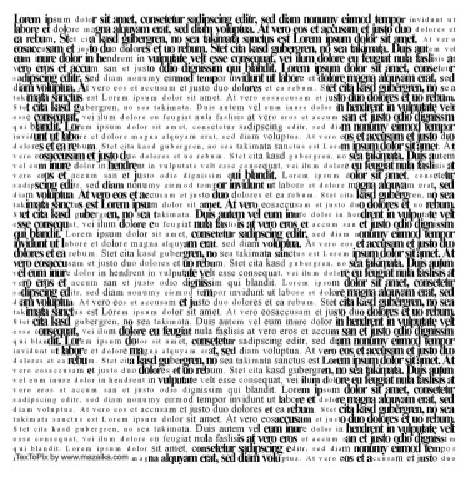
\includegraphics[width=0.5\textwidth]{Greenhill_Subrahmanyan/01x01-eps-converted-to}
\end{center}
\caption{This is figure 1 in chapter 1.}
\end{figure}

\paragraph{Cras adipiscing} sagittis nunc vel luctus. Suspendisse volutpat augue quis erat semper consequat dignissim tellus euismod. Morbi hendrerit, tellus id aliquam iaculis, nibh leo tincidunt eros, vitae varius ligula felis in mi.

\begin{table}
\caption{Greek Letters.}
\begin{center}
\begin{tabular}{llllllll}
\hline
$\alpha $  & $ \beta $  & $ \gamma $  & $ \delta $  & $ \epsilon $  & $ \varepsilon $  & $ \zeta $  & $ \eta $ \\
 $ \theta $  &  $ \vartheta $  &  $ \gamma $  &  $ \kappa $  &  $ \lambda $  &  $ \mu $  &  $ \nu $  &  $ \xi $ \\
 $ o $  &  $ \pi $  &  $ \varpi $  &  $ \rho $  &  $ \varrho $  &  $ \sigma $  &  $ \varsigma $  &  $$ \\
 $ \tau $  &  $ \upsilon $  &  $ \phi$ &  $ \varphi $  &  $ \chi $  &  $ \psi $  &  $ \omega$  &  $ $ \\
 &  &  &  &  &  &  & \\
$ \Gamma $  & $ \Delta $  & $ \Theta $  &  $ \Lambda $  &  $ \Xi $  &  $ \Pi $  &  $ \Sigma $  & $ \Upsilon $ \\
 $ \Phi$ &  $ \Psi $  &  $ \Omega $  &  &  &  &  &\\
\hline
\end{tabular}
\end{center}\end{table}

\begin{figure}[]
\begin{center}
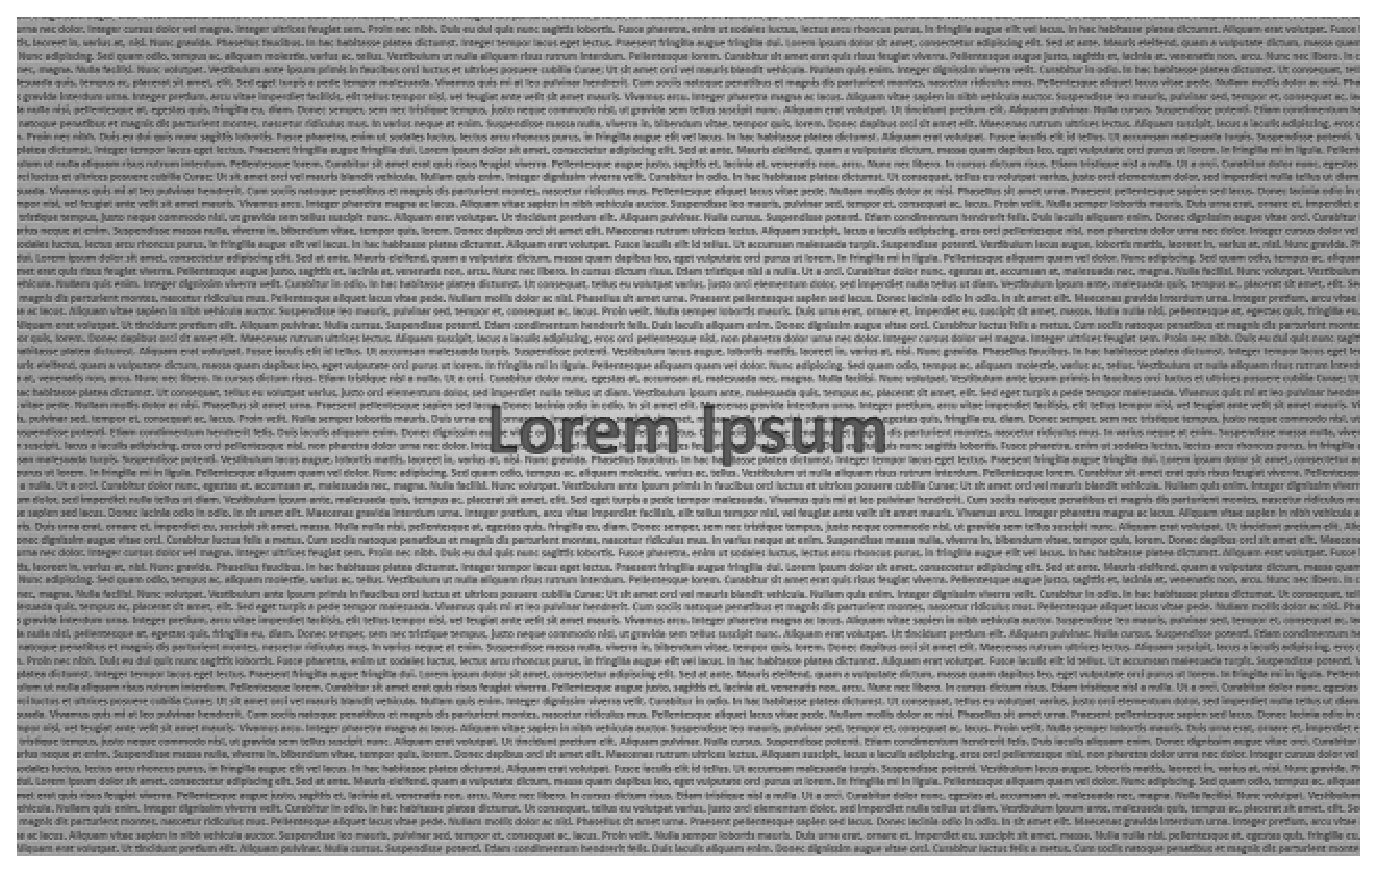
\includegraphics[width=0.6\textwidth]{Greenhill_Subrahmanyan/01x02}
\end{center}
\caption{This is figure 2 in chapter 1.}
\end{figure}


\bibliographystyle{plain}
\bibliography{Greenhill_Subrahmanyan/References}


